\documentclass[journal=jctc,manuscript=article,preprint]{achemso}
\usepackage[version=3]{mhchem} % Formula subscripts using \ce{}
\usepackage{caption}
\usepackage{subcaption}
\usepackage{hyperref}
\usepackage{natbib}
\usepackage{siunitx}
\usepackage{tabularx}
\usepackage{amsmath}
\usepackage{xcolor}

\newcommand*\mycommand[1]{\texttt{\emph{#1}}}
\newcommand{\Iaq}{{I\alpha,\mathbf{q}}}
\newcommand{\Jbq}{{J\beta,\mathbf{q}}}
\newcommand{\bfk}{{\mathbf{k}}}
\newcommand{\bfq}{{\mathbf{q}}}
\newcommand{\bfG}{{\mathbf{G}}}
\newcommand{\bfr}{{\mathbf{r}}}


\author{Han Yang}
\affiliation{Department of Chemistry, University of Chicago, Chicago, Illinois 60637, United States}
\alsoaffiliation{Pritzker School of Molecular Engineering, The University of Chicago, Chicago, Illinois 60637, United States}
\author{Marco Govoni}
\affiliation{Materials Science Division and Center for Molecular Engineering, Argonne National Laboratory, Lemont, Illinois 60439, United States}
\alsoaffiliation{Pritzker School of Molecular Engineering, The University of Chicago, Chicago, Illinois 60637, United States}
\email{mgovoni@anl.gov}
\author{Arpan Kundu}
\affiliation{Pritzker School of Molecular Engineering, The University of Chicago, Chicago, Illinois 60637, United States}
\author{Giulia Galli}
\affiliation{Department of Chemistry, University of Chicago, Chicago, Illinois 60637, United States}
\alsoaffiliation{Pritzker School of Molecular Engineering, The University of Chicago, Chicago, Illinois 60637, United States}
\alsoaffiliation{Materials Science Division and Center for Molecular Engineering, Argonne National Laboratory, Lemont, Illinois 60439, United States}
\email{gagalli@uchicago.edu}

\title{Supplementary Information: Combined first-principles calculations of electron-electron and electron-phonon self-energies in condensed systems}
\begin{document}
\maketitle

\section{Evaluation of electron-phonon self-energies with the Lanczos approach}

We discuss an approach based on the Lanczos method\cite{lanczos1950iteration}, to avoid summation over empty bands when computing the electron-phonon self-energy.
Staring from Eq.~17 of the main text, we define $A_{n\mathbf{k}}(\tilde{H}_{\mathbf{k}+\mathbf{q}}) = (\varepsilon_{n\bfk}-\tilde{H}_{\bfk+\bfq})^{-1}$, and Eq.~17 can be written as,
\begin{equation}
    A_{n\bfk}(\tilde{H}_{\bfk+\bfq}) = \sum_{m}\left|\psi_{m\bfk+\bfq}\right\rangle A_{n\bfk}(\varepsilon_{m\bfk+\bfq})\left\langle\psi_{m\bfk+\bfq}\right|
\end{equation}

Following references\cite{lanczos1950iteration,mcavoy2018coupling}, we obtain the Lanczos basis $\tilde{q}_l$ and corresponding eigenvalues $d_l$ of $\tilde{H}_{\bfk+\bfq}$, and thus the self-energy can be written as
\begin{equation}
    \Sigma_{n\bfk}^{FM}(T) = \sum_{\nu\bfq l}\left\langle L_{n\bfk}^{\bfq\nu} |\tilde{q}_{l}\right\rangle A_{n\bfk}(d_l)\left\langle \tilde{q}_l | R_{n\bfk}^{\bfq\nu} \right\rangle[2n_{\bfq\nu}(T)+1],\label{equ:FM_Lanczos}
\end{equation}
where $\left| L_{n\bfk}^{\bfq\nu} \right\rangle$ and $\left| R_{n\bfk}^{\bfq\nu} \right\rangle$ are vectors within the set $\{\left|\partial_{\bfq\nu}V_{SCF}\psi_{n\bfk}\right\rangle,\,n = 1,\,2,\,\cdots\}$.

In the following, we describe how to compute Lanczos basis functions, and hereafter we drop the superscripts and subscripts of $\left|L\right\rangle$ and $\left|R\right\rangle$ for simplicity. The Lanczos basis functions and eigenvalues can be obtained by diagonalizing the matrix
\begin{equation}
    Q^\dagger\tilde{H}Q = \left(
    \begin{matrix}
    \alpha_1 &  \beta_2 &          &         &          \\
    \beta_2  & \alpha_2 &  \beta_3 &         &          \\
             & \beta_3  & \ddots   & \ddots  &          \\
             &          & \ddots   & \ddots  & \beta_n  \\
             &          &          & \beta_n & \alpha_n \\
    \end{matrix}
    \right)
    \label{equ:Lanczos_matrix}
\end{equation}
where $Q = \{\left|q_l\right\rangle,\,l\,=\,1,\,2,\,\cdots,\,N_\mathrm{Lanczos}\}$ with $\left|q_1\right\rangle = \left|R\right\rangle$ are a set of orthonomal vectors, and the elements of the matrix are obtained from
\begin{equation}
    \alpha_n = \left\langle q_l \left| \tilde{H} \right| q_l\right\rangle
\end{equation}
and
\begin{equation}
    \beta_{n+1} = ||(\tilde{H}-\alpha_n)\left|q_n\right\rangle-\beta_n\left|q_{n-1}\right\rangle|| .
\end{equation}
The vectors  $\left|q_l \right\rangle$ are orthogonalized  with a recursive process by applying
\begin{equation}
    \left|q_{n+1}\right\rangle = \frac{1}{\beta_{n+1}}\left[(\tilde{H}-\alpha_n)\left|q_n\right\rangle-\beta_n\left|q_{n-1}\right\rangle\right].
\end{equation}
The diagonalization of Eq.~\ref{equ:Lanczos_matrix} yields the eigenvalues $d_l$ and corresponding eigenvectors $U_l$. We then define a modified basis set $\left| \tilde{q}_l \right\rangle$ as a linear combination of the original basis $\left| q_l \right\rangle$,
\begin{equation}
    \left| \tilde{q}_l \right\rangle  = \sum_{k}^{N_\mathrm{Lanczos}} U_l^k\left|q_k \right\rangle.
\end{equation}
Having obtained the eigenvalues $d_l$ of the matrix $Q^\dagger\tilde{H}Q$ and using the modified basis $\left| \tilde{q}_l \right\rangle$, we can evaluate the Fan-Migdal self-energy in Eq.~\ref{equ:FM_Lanczos}, without summations over empty bands. A similar technique can  be applied to obtain the Debye-Waller self-energy.

In addition, we can compute the temperature-dependent, non-adiabatic or frequency-dependent self-energies without any extra computational cost, by reusing the Lanczos basis set defined above. 


\section{Convergence study of phonon frequencies in diamond}

To verify our implementation, we computed phonon frequencies with the method described in the main text with the LDA functional and 60 Ry cutoff, and compared them with the results obtained with the \texttt{PHonon}\cite{giannozzi2009quantum} code.
Fig.~\ref{fig:diamond_dispersion} shows the phonon dispersion curves computed with our code and the \texttt{PHonon} code, which are indistinguishable.

We also carried out additional  comparisons with higher energy cutoffs and in Fig.~\ref{fig:phonon_differences} we report the differences of the phonon frequencies with different energy cutoffs. As the energy cutoff increases, both methods converge to the same phonon frequencies. 
\begin{figure}
    \centering
    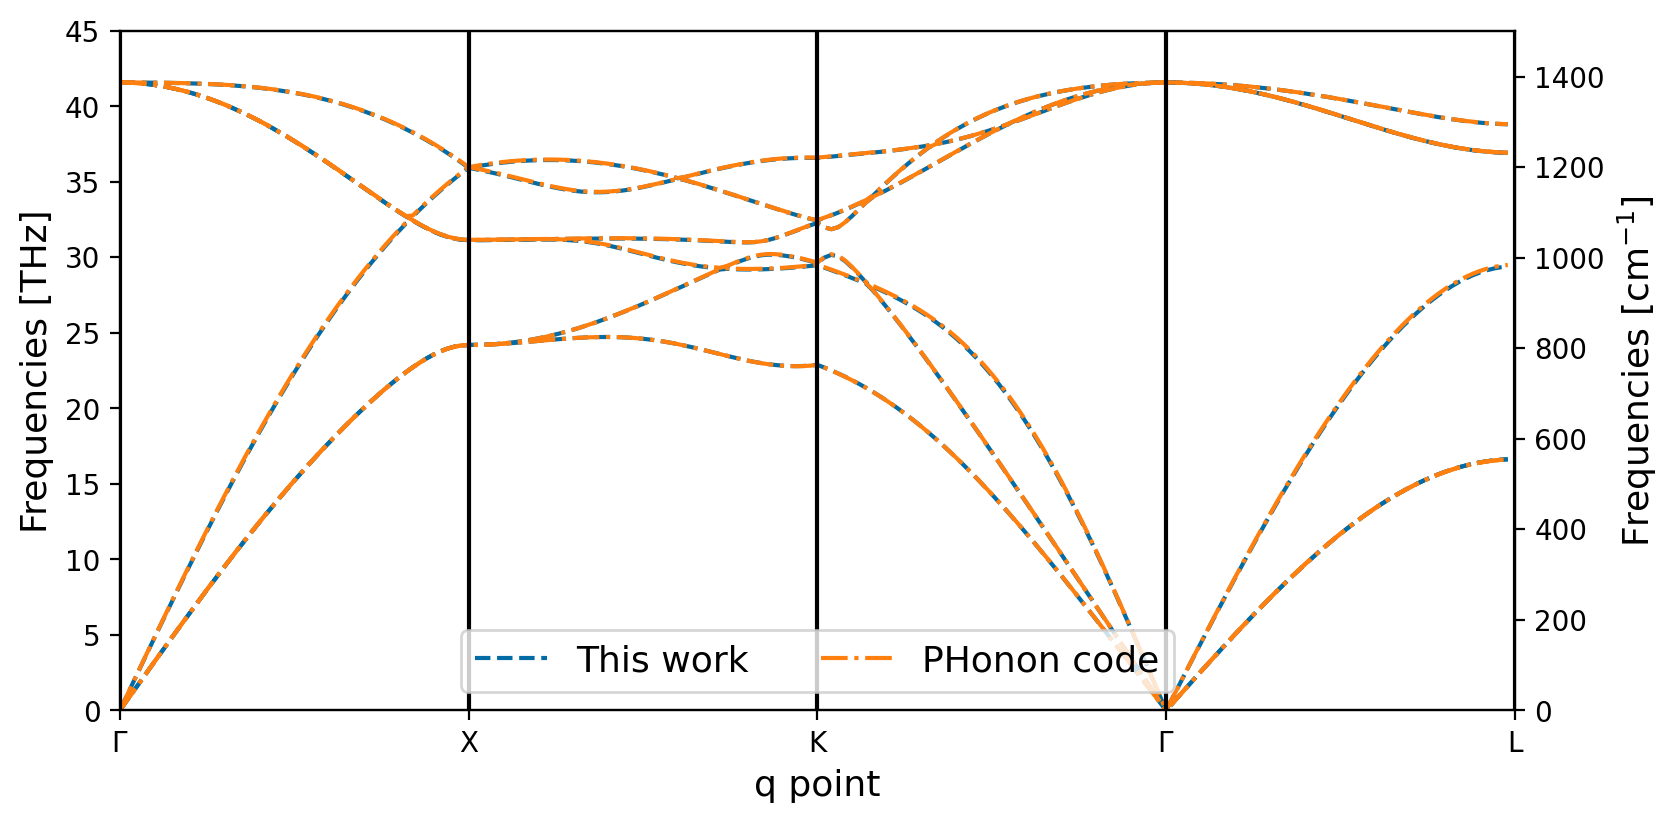
\includegraphics[width=0.8\textwidth]{fig/Diamond_phonon_dispersion_60Ry.png}
    \caption{Phonon dispersion of diamond interpolated from $3\times3\times3$ $\bfq$-point sampling. A kinetic energy cutoff of 60 Ry and LDA functional were used. }
    \label{fig:diamond_dispersion}
\end{figure}

\begin{figure}
    \centering
    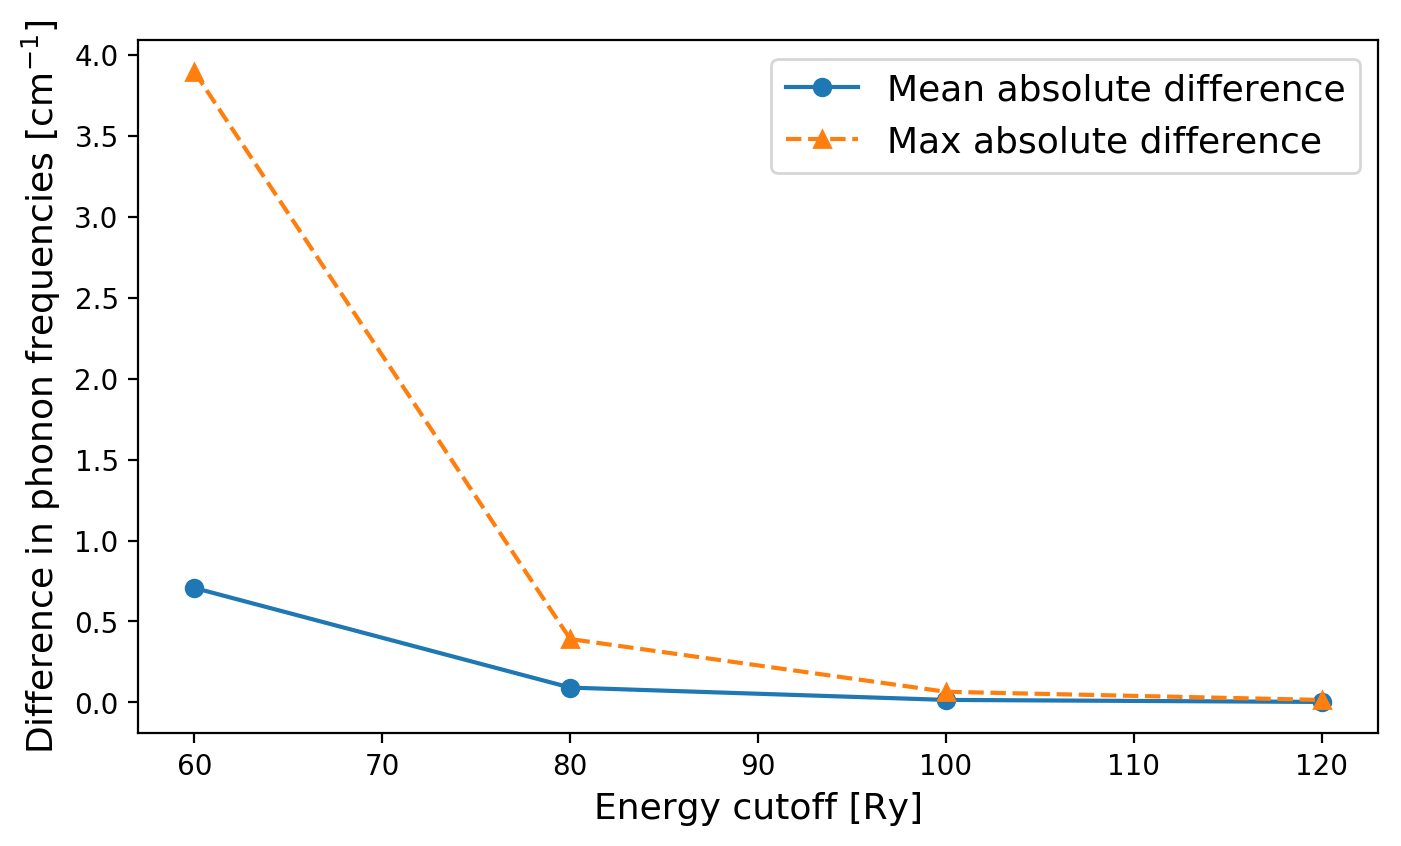
\includegraphics[width=0.8\textwidth]{fig/Diamond_phonon_differences.png}
    \caption{Mean and maximum absolute difference of phonon frequencies [in $\mathrm{cm}^{-1}$] computed with the method discussed in this work and the \texttt{PHonon} package in \texttt{Quantum Espresso}.}
    \label{fig:phonon_differences}
\end{figure}

\clearpage

\section{ Numerical protocol used in Table 3 of the main text}
The $G_0W_0$ self-energy $\Sigma$ contains an exchange term 
\begin{equation}
    \Sigma_x(\bfr,\bfr^\prime) = -\sum_{n=1}^{N_\mathrm{occ}}\sum_{\bfk}\psi_{n\bfk}(\bfr)v_c(\bfr,\bfr^\prime)\psi_{n\bfk}^*(\bfr^\prime)
\end{equation}
and a correlation term
\begin{equation}
    \Sigma_c(\bfr,\bfr^\prime;\omega) = i\int_{-\infty}^{+\infty}\frac{\mathrm{d}\omega^\prime}{2\pi}G_\mathrm{KS}(\bfr,\bfr^\prime;\omega+\omega^\prime)W_p(\bfr,\bfr^\prime;\omega^\prime),
\end{equation}  
where $\psi_{n\bfk}$ are Kohn-Sham orbitals associated with the $n$-th level at the $\bfk$ point, $v_c$ is the bare Coulomb potential, $G_\mathrm{KS}$ is the Green function written in terms of Kohn-Sham orbitals,
\begin{equation}
    G_\mathrm{KS}(\bfr,\bfr^\prime,\omega) = \sum_{n\bfk}\frac{\psi_{n\bfk}(\bfr)\psi^*_{n\bfk}(\bfr^\prime)}{\omega-\varepsilon_{n\bfk}}
\end{equation}
with $\varepsilon_{n\bfk}$ being the $n$-th Kohn-Sham energy at the $\bfk$ point, and $W_p$ is the difference between the screened Coulomb potential and bare Coulomb potential,
\begin{equation}
    W_p(\bfr,\bfr^\prime;\omega) = W(\bfr,\bfr^\prime;\omega) - v_c(\bfr,\bfr^\prime)
\end{equation}

To improve the convergence of the calculations of the exchange part $\Sigma_x$ with respect to the number of $\bfk$ points, the curvature technique developed by  Gygi-Baldereschi\cite{Gygi1986} and further refined by   Ref.~\citenum{nguyen2009efficient} was used in most of our calculations. In Table 3 of the main text, the curvature technique is used to obtain the results presented in P1 and P2, but not those of P3 -- P5.

The screened Coulomb interaction $W$ is evaluated by computing  the dielectric matrix $\epsilon$,
\begin{equation}
    W(\bfr,\bfr^\prime;\omega) = \epsilon^{-1}(\bfr,\bfr^\prime;\omega)v_c(\bfr,\bfr^\prime).
\end{equation}
and the symmetrized dielectric matrix $\tilde{\epsilon}$ is computed from the symmetrized polarizibility $\tilde{\chi}^0$,
\begin{equation}
    \tilde{\epsilon}_{\bfG\bfG^\prime}(\bfq,\omega) = \delta_{\bfG\bfG^\prime} - \tilde{\chi}^0_{\bfG\bfG^\prime}(\bfq,\omega).
\end{equation}
The symmetrized polarizibility can be written as:
\begin{equation}
\begin{aligned}
    \tilde{\chi}^0_{\bfG\bfG^\prime}(\bfq;\omega) = & -4\pi e^2\sum_n^{N_\mathrm{occ}}\sum_{m=N_\mathrm{occ}+1}^{+\infty}\sum_\bfk  \frac{\rho^*_{mn\bfk}(\bfq,\bfG)\rho_{jmn\bfk}(\bfq,\bfG^\prime)}{|\bfq+\bfG||\bfq+\bfG^\prime|} \\
    & \times\left[ \frac{1}{\varepsilon_{m\bfk}-\varepsilon_{n\bfk-\bfq}+\omega-i0^+} + \frac{1}{\varepsilon_{m\bfk}-\varepsilon_{n\bfk-\bfq}-\omega-i0^+}
    \right]
\end{aligned}
\end{equation}
with
\begin{equation}
    \rho_{mn\bfk}(\bfq,\bfG) = \left\langle \psi_{m\bfk} \left| \mathbf{e}^{i(\bfq+\bfG)\cdot\bfr}\right|\psi_{n\bfk-\bfq}\right\rangle
\end{equation}

The straightforward evaluation of the polarizibility $\tilde{\chi}^0$ is expensive because it requires the summation over empty bands and it is frequency dependent. In Table 3 of the main text, the calculations presented in the last column used 100 states for  the summation over empty bands. To compare our results with those if the literature, we also used 100 states for the results given in columns P2 -- P5. By using the Lanczos algorithm, we can avoid the summation over empty bands and there is no need to truncate the summation. For the results of the P1 column, only 8 bands are used, and we show  that the Lanczos algorithm yields the same result as that of the P2 column, where 100 bands are used.

In Table 3 of the main text, the calculation shown in the last column used the Plasmon-Pole model (PPM),\cite{ppm1986} a semi-empirical model, to compute the frequency dependence of the dielectric matrix, but our $G_0W_0$ calculation computes the full frequency (FF) dependence using the Lanczos approach without using any semi-empirical approximations. To compare our results with those existing in the literature, we used the PPM in column P5 and we did reproduce the literature result. However, FF is known to be more accurate than the PPM,\cite{golze2019gw} thus we used FF in obtaining the results of P1 -- P4.

The calculation of electron-phonon self-eneriges also requires to carry out  summations over empty bands, and we used the Lanczos technique for the electron-phonon self-energies in column P1 -- P5.

More details on the implementation of the $G_0W_0$ approximation can be found in Ref.~\citenum{govoni2015large}.

\section{Pseudopotentials used in this paper}
In \autoref{tab:Pseudopotentials}, we list the pseudopotentials that were used in this work.
\begin{table}[]
    \centering
    \begin{tabularx}{\textwidth}{lX}
    \hline\hline
    Pseudopotential & Comment  \\
    \hline
    C.pz-mt.fhi.UPF  & Martins-Troullier\cite{troullier1991efficient} type pseudopotential of carbon generated with Perdew-Zunger\cite{perdew1981self} parameterized LDA functional in UPF format and is ready for \texttt{Quantum Espresso} calculation. \\
    \hline
    C.pz-mt.fhi & Martins-Troullier\cite{troullier1991efficient} type pseudopotential of carbon generated with Perdew-Zunger\cite{perdew1981self} parameterized LDA functional in fhi format and is ready for \texttt{ABINIT} calculation. \\
    \hline
    C\_ONCV\_PBE-1.0.upf & SG15\cite{schlipf2015SG15} ONCV\cite{hamann2013ONCV} pseudopotential of carbon generated with PBE functional\cite{perdew1996PBE} and is ready for \texttt{Quantum Espresso} calculation. \\
    \hline
    B\_ONCV\_PBE-1.0.upf & SG15\cite{schlipf2015SG15} ONCV\cite{hamann2013ONCV} pseudopotential of boron generated with PBE functional\cite{perdew1996PBE} and is ready for \texttt{Quantum Espresso} calculation.\\
    \hline
    N\_ONCV\_PBE-1.0.upf & SG15\cite{schlipf2015SG15} ONCV\cite{hamann2013ONCV} pseudopotential of nitrogen generated with PBE functional\cite{perdew1996PBE} and is ready for \texttt{Quantum Espresso} calculation.\\
    \hline\hline
    \end{tabularx}
    \caption{Pseudopotentials used in this paper}
    \label{tab:Pseudopotentials}
\end{table}
\clearpage
\bibliography{ref.bib}
\end{document}